\section{INTRODUCTION}

\subsection{Motivation}
Dynamic traffic routing provides drivers with route recommendations based on real-time road information. It has been used as one of  promising control policies for alleviating congestion  \cite{como2012robust_2, minh2022effective}, and is expected to find extensive applications in a connected vehicle environment \cite{han2020congestion, chen2021distributed}. Nevertheless, it is also reported that driver non-compliance with route guidance could undermine the performance of dynamic routing \cite{powell2000value}, especially social routing advice that deliberately detours part of vehicles to achieve benefits in terms of road networks \cite{van2019travelers}. Although more and more surveys have confirmed this disobedience \cite{dia2007modelling,kerkman2012car,djavadian2014empirical,van2020travelers, mariotte2021assessing}, limited studies have investigated in an analytical way how drivers' adherence influences the effect of traffic routing control.

In this paper, we focus on routing advice released by traffic system operators/agencies. We study the above problem by considering a setting with random demand and random driver non-compliance. We analyze the resulting stochastic dynamical system under  routing control. Specially, we focus on a network comprised of two parallel links; see Fig.~\ref{fig_twolink}. Though simple, the two-link network serves as a typical scenario for studying routing control \cite{ephremides1980simple, zhang2019modeling,xie2020resilience,tang2020security}; it turns out to be an appropriate abstraction of multiple parallel links: one stands for arterials and the other denotes a set of local streets \cite{pi2017stochastic}. Furthermore, we adopt a Markov chain to model the compliance rate that possibly depends on traffic states. It allows us to study stability and instability criteria that determine whether the network is destabilized by the random compliance rate. We also quantify the impacts of drivers' disobedience in terms of throughput, namely the maximum constant inflow under which the network can be stabilized.
\begin{figure}[htbp]
    \centering
    \begin{tikzpicture}
        %Vertex
        \Vertex[x=-3,style={color=white}]{A}
        \Vertex[x=0, style=black, size=0.1]{B}
        \Vertex[x=4, style=black, size=0.1]{N}
        %Edge
        \Edge[Direct, label={demand $D(t)$}](A)(B)
        \Edge[Direct,bend=30, label={major link $e_1$}](B)(N)
        \Edge[Direct,bend=330, label={minor link $e_2$}](B)(N)
        
        %Text
        \Text[x=-0.3,y=-0.4, fontsize=\footnotesize]{Origin}
        \Text[x=4.3,y=-0.4, fontsize=\footnotesize]{Destination}
    \end{tikzpicture}
    \caption{The two-link network.}
    \label{fig_twolink}
\end{figure}

\subsection{Related work}

Previous work on evaluating impacts of the conformity with routing advice typically applied static or dynamic traffic assignment (STA or DTA). These methods are favored since they easily provide numerical assessment in terms of efficiency, equity and so on \cite{van2019travelers, zhang2019modeling,ning2023robust} and can be implemented even for large-scale networks.  However, they also have disadvantages. STA finds equilibrium by solving mathematical programming. It fails to capture significant traffic dynamics, such as congestion spillback and fluctuations of drivers' compliance rate and thus could induce unrealistic equilibrium. Though DTA can address the shortcomings of STA to some extent, it introduces a new problem. As we see later, low compliance rates could make traffic networks unstable. In that case, it could be problematic to apply DTA since we do not have guaranteed convergence in advance. Noting this, we aim at developing methods that allow stability and instability analysis, at least in some conditions, before numerical evaluation. To our best knowledge, limited studies discussed this topic for routing control subject to random compliance.

%Previous work on the conformity with routing advice can be categorized into three parts. The first part explored the factors in drivers' willingness to follow the guidance, including expected travel time/delay, trip purposes and so on 

%The second part evaluated performance of routing control subject to heterogeneous drivers' choice behavior, typically using static or dynamic traffic assignment (STA or DTA) . STA finds equilibrium by solving mathematical programming. It ignores significant dynamics, such as congestion spillback and fluctuations of compliance rates and thus could induce unreliable equilibrium. Though DTA can address the shortcomings of STA to some extent, 

%There are also a few studies involving optimal design of routing control in presence of the non-compliance \cite{pi2017stochastic,paz2009behavior, weymann1995dynamic}. Although.

Our model belongs to discrete-time nonlinear stochastic systems. Although the general theories of stochastic stability have been studied extensively \cite{berman2006h,zhang2016lasalle, zhang2021robust,meyn1993survey,meyn2012markov}, how to apply them in our problem is still unclear. Typically, stability analysis can be refined for specific non-linear systems. Besides, it should be noted that most of studies mainly discuss sufficient stability conditions for general nonlinear stochastic systems, while we also have interest in instability conditions.

\subsection{Our contributions}

In this paper we address the two following questions:
\begin{enumerate}
    \item How to determine whether the network can be stabilized by routing control subject to driver non-compliance?
    \item How to evaluate efficiency losses of routing control due to the non-compliance in an analytic way?
\end{enumerate}

We answer the first question for two types of networks. In the first one, the two parallel links have infinite space and there are no congestion spillback, while in the second one, the two parallel links with finite space may. We formulate discrete-time nonlinear stochastic systems for the two networks, respectively. Then we apply the Foster-Lyapunov criteria \cite{meyn2012markov} to derive the stability condition and scrutinize transience of Markov chains \cite{meyn2012markov,meyn1993survey} to obtain instability conditions. For the first network, we successfully obtain a sufficient and necessary stability condition (Theorem~\ref{thm_1}); for the second one, we have one stability crietrion (Theorems \ref{thm_2}) and one instability criterion (Theorems \ref{thm_3}). 

Even when the network is stable, we want to know to what extent the network performance decrease. Thus to answer the second question, we take throughput as the metric to measure efficiency losses. However, throughput is not always available even for the two-link network. For the two links with infinite buffer sizes, we indeed derive exact values of throughput since we have a sufficient and necessary stability condition. For the two links with finite buffer sizes, we use the stability and instability conditions to yield lower and upper bounds, respectively.  

The rest of the paper is organized as follows. Section~\ref{sec_modeling} introduces our modeling framework.
Section~\ref{sec_stability} presents the results when the two parallel links have infinite storage space, and Section~\ref{sec_example} provides the results in case of two links with limited buffer sizes. Finally, Section~\ref{sec_conclusion} summarizes our work and discusses future research.

%\begin{table}
%\caption{An Example of a Table}
%\label{table_example}
%\begin{center}
%\begin{tabular}{|c||c|}
%\hline
%One & Two\\
%\hline
%Three & Four\\
%\hline
%\end{tabular}
%\end{center}
%\end{table}